\documentclass{formation}

\title{Réseaux de neurones à convolutions}

\begin{document}

\maketitle

\begin{frame}
  \frametitle{Objectifs}
  \begin{itemize}
  \item Appliquer les réseaux de neurones aux images
  \item Comprendre le mécanisme des convolutions
  \item Connaître les couches liées aux convolutions
  \end{itemize}
\end{frame}

\begin{frame}
  \frametitle{Limitations des réseaux denses pour les images}
  Principale faiblesse: chaque input est spécifique pour les poids
  appris.

  → Impossible de gérer efficacement les translations\\
  → Impossible
  d'appliquer un neurone détectant une forme à une autre position dans
  l'image

  \alert{On pallie ces problèmes avec les réseaux à convolutions.}
\end{frame}

\begin{frame}
  \frametitle{Réseaux à convolutions}
  Idées fortes:

  \begin{itemize}
  \item Restreindre l'input des neurones
  \item Appliquer un même neurone à plusieurs zones restreintes
  \end{itemize}
\end{frame}

\begin{frame}
  \frametitle{Neurone dans un réseau à convolutions}
  \begin{itemize}
  \item Appelé filtre ou kernel
  \item Réceptionne souvent entre 1x1 et 7x7 inputs seulement
  \item Appliqué plusieurs fois au lieu d'une seule
  \item Un même neurone a donc \alert{plusieurs outputs}.
  \end{itemize}
\end{frame}

\begin{frame}
  \frametitle{Application d'un filtre}
  \begin{multicols}{2}
    Image:
    \begin{tabular}{|c|c|c|c|}
      \hline
      1 & 2 & 0 & 5 \\
      \hline
      3 & 1 & 0 & -1 \\
      \hline
      0 & 3 & 0 & 1 \\
      \hline
      0 & 4 & 5 & 5 \\
      \hline
    \end{tabular}

    \columnbreak

    Filtre:
    \begin{tabular}{|c|c|}
      \hline
      0 & 1 \\
      \hline
      2 & -1 \\
      \hline
    \end{tabular}
    \vfill
  \end{multicols}
  Application successive du filtre sur les différentes zones de l'image
\end{frame}

\begin{frame}
  \frametitle{Application d'un filtre}
  \begin{multicols}{2}
    Image:
    \begin{tabular}{|c|c|c|c|}
      \hline
      \cellcolor{green}1 & \cellcolor{green}2 & 0 & 5 \\
      \hline
      \cellcolor{green}3 & \cellcolor{green}1 & 0 & -1 \\
      \hline
      0 & 3 & 0 & 1 \\
      \hline
      0 & 4 & 5 & 5 \\
      \hline
    \end{tabular}

    \columnbreak

    Filtre:
    \begin{tabular}{|c|c|}
      \hline
      0 & 1  \\
      \hline
      2 & -1 \\
      \hline
    \end{tabular}\\[.5cm]
    Résultat:
    \begin{tabular}{|c|c|c|}
      \hline
      7 & \phantom{6} & \phantom{-2} \\
      \hline
       \phantom{-2}  &  & \\
      \hline
        &  & \\
      \hline
    \end{tabular}
  \end{multicols}
  Application successive du filtre sur les différentes zones de l'image
\end{frame}
\begin{frame}
  \frametitle{Application d'un filtre}
  \begin{multicols}{2}
    Image:
    \begin{tabular}{|c|c|c|c|}
      \hline
      1 & \cellcolor{green}2 & \cellcolor{green}0 & 5 \\
      \hline
      3 & \cellcolor{green}1 & \cellcolor{green}0 & -1 \\
      \hline
      0 & 3 & 0 & 1 \\
      \hline
      0 & 4 & 5 & 5 \\
      \hline
    \end{tabular}

    \columnbreak

    Filtre:
    \begin{tabular}{|c|c|}
      \hline
      0 & 1  \\
      \hline
      2 & -1 \\
      \hline
    \end{tabular}\\[.5cm]
    Résultat:
    \begin{tabular}{|c|c|c|}
      \hline
      7 & 2 & \phantom{-2} \\
      \hline
       \phantom{-2}  &  & \\
      \hline
        &  & \\
      \hline
    \end{tabular}
  \end{multicols}
  Application successive du filtre sur les différentes zones de l'image
\end{frame}
\begin{frame}
  \frametitle{Application d'un filtre}
  \begin{multicols}{2}
    Image:
    \begin{tabular}{|c|c|c|c|}
      \hline
      1 & 2 & \cellcolor{green}0 & \cellcolor{green}5 \\
      \hline
      3 & 1 & \cellcolor{green}0 & \cellcolor{green}-1 \\
      \hline
      0 & 3 & 0 & 1 \\
      \hline
      0 & 4 & 5 & 5 \\
      \hline
    \end{tabular}

    \columnbreak

    Filtre:
    \begin{tabular}{|c|c|}
      \hline
      0 & 1  \\
      \hline
      2 & -1 \\
      \hline
    \end{tabular}\\[.5cm]
    Résultat:
    \begin{tabular}{|c|c|c|}
      \hline
      7 & 2 & 6\\
      \hline
       \phantom{-2} &  & \phantom{-2} \\
      \hline
        &  & \\
      \hline
    \end{tabular}
  \end{multicols}
  Application successive du filtre sur les différentes zones de l'image
\end{frame}

\begin{frame}
  \frametitle{Application d'un filtre}
  \begin{multicols}{2}
    Image:
    \begin{tabular}{|c|c|c|c|}
      \hline
      1 & 2 & 0 & 5 \\
      \hline
      \cellcolor{green}3 & \cellcolor{green}1 & 0 & -1 \\
      \hline
      \cellcolor{green}0 & \cellcolor{green}3 & 0 & 1 \\
      \hline
      0 & 4 & 5 & 5 \\
      \hline
    \end{tabular}

    \columnbreak

    Filtre:
    \begin{tabular}{|c|c|}
      \hline
      0 & 1  \\
      \hline
      2 & -1 \\
      \hline
    \end{tabular}\\[.5cm]
    Résultat:
    \begin{tabular}{|c|c|c|}
      \hline
      7 & 2 & 6\\
      \hline
      -2 &  & \phantom{-2}\\
      \hline
        &  & \\
      \hline
    \end{tabular}
  \end{multicols}
  Application successive du filtre sur les différentes zones de l'image
\end{frame}

\begin{frame}
  \frametitle{Application d'un filtre}
  \begin{multicols}{2}
    Image:
    \begin{tabular}{|c|c|c|c|}
      \hline
      1 & 2 & 0 & 5 \\
      \hline
      3 & \cellcolor{green}1 & \cellcolor{green}0 & -1 \\
      \hline
      0 & \cellcolor{green}3 & \cellcolor{green}0 & 1 \\
      \hline
      0 & 4 & 5 & 5 \\
      \hline
    \end{tabular}

    \columnbreak

    Filtre:
    \begin{tabular}{|c|c|}
      \hline
      0 & 1  \\
      \hline
      2 & -1 \\
      \hline
    \end{tabular}\\[.5cm]
    Résultat:
    \begin{tabular}{|c|c|c|}
      \hline
      7 & 2 & 6\\
      \hline
      -2 & 6 &  \phantom{-2}\\
      \hline
        &  & \\
      \hline
    \end{tabular}
  \end{multicols}
  Application successive du filtre sur les différentes zones de l'image
\end{frame}

\begin{frame}
  \frametitle{Application d'un filtre}
  \begin{multicols}{2}
    Image:
    \begin{tabular}{|c|c|c|c|}
      \hline
      1 & 2 & 0 & 5 \\
      \hline
      3 & 1 & \cellcolor{green}0 & \cellcolor{green}-1 \\
      \hline
      0 & 3 & \cellcolor{green}0 & \cellcolor{green}1 \\
      \hline
      0 & 4 & 5 & 5 \\
      \hline
    \end{tabular}

    \columnbreak

    Filtre:
    \begin{tabular}{|c|c|}
      \hline
      0 & 1  \\
      \hline
      2 & -1 \\
      \hline
    \end{tabular}\\[.5cm]
    Résultat:
    \begin{tabular}{|c|c|c|}
      \hline
      7 & 2 & 6\\
      \hline
      -2 & 6 & -2\\
      \hline
        &  & \\
      \hline
    \end{tabular}
  \end{multicols}
  Application successive du filtre sur les différentes zones de l'image
\end{frame}

\begin{frame}
  \frametitle{Application d'un filtre}
  \begin{multicols}{2}
    Image:
    \begin{tabular}{|c|c|c|c|}
      \hline
      1 & 2 & 0 & 5 \\
      \hline
      3 & 1 & 0 & -1 \\
      \hline
      \cellcolor{green}0 & \cellcolor{green}3 & 0 & 1 \\
      \hline
      \cellcolor{green}0 & \cellcolor{green}4 & 5 & 5 \\
      \hline
    \end{tabular}

    \columnbreak

    Filtre:
    \begin{tabular}{|c|c|}
      \hline
      0 & 1  \\
      \hline
      2 & -1 \\
      \hline
    \end{tabular}\\[.5cm]
    Résultat:
    \begin{tabular}{|c|c|c|}
      \hline
      7 & 2 & 6\\
      \hline
      -2 & 6 & -2\\
      \hline
      -1 &  & \\
      \hline
    \end{tabular}
  \end{multicols}
  Application successive du filtre sur les différentes zones de l'image
\end{frame}

\begin{frame}
  \frametitle{Application d'un filtre}
  \begin{multicols}{2}
    Image:
    \begin{tabular}{|c|c|c|c|}
      \hline
      1 & 2 & 0 & 5 \\
      \hline
      3 & 1 & 0 & -1 \\
      \hline
      0 & \cellcolor{green}3 & \cellcolor{green}0 & 1 \\
      \hline
      0 & \cellcolor{green}4 & \cellcolor{green}5 & 5 \\
      \hline
    \end{tabular}

    \columnbreak

    Filtre:
    \begin{tabular}{|c|c|}
      \hline
      0 & 1  \\
      \hline
      2 & -1 \\
      \hline
    \end{tabular}\\[.5cm]
    Résultat:
    \begin{tabular}{|c|c|c|}
      \hline
      7 & 2 & 6\\
      \hline
      -2 & 6 & -2\\
      \hline
      -1 & 3 & \\
      \hline
    \end{tabular}
  \end{multicols}
  Application successive du filtre sur les différentes zones de l'image
\end{frame}

\begin{frame}
  \frametitle{Application d'un filtre}
  \begin{multicols}{2}
    Image:
    \begin{tabular}{|c|c|c|c|}
      \hline
      1 & 2 & 0 & 5 \\
      \hline
      3 & 1 & 0 & -1 \\
      \hline
      0 & 3 & \cellcolor{green}0 & \cellcolor{green}1 \\
      \hline
      0 & 4 & \cellcolor{green}5 & \cellcolor{green}5 \\
      \hline
    \end{tabular}

    \columnbreak

    Filtre:
    \begin{tabular}{|c|c|}
      \hline
      0 & 1  \\
      \hline
      2 & -1 \\
      \hline
    \end{tabular}\\[.5cm]
    Résultat:
    \begin{tabular}{|c|c|c|}
      \hline
      7 & 2 & 6\\
      \hline
      -2 & 6 & -2\\
      \hline
      -1 & 3 & 6\\
      \hline
    \end{tabular}
  \end{multicols}
  Application successive du filtre sur les différentes zones de l'image
\end{frame}

\begin{frame}
  \frametitle{Exercice}
  \begin{multicols}{2}
    Image:
    \begin{tabular}{|c|c|c|c|}
      \hline
      3 & 2 & -2 & -3 \\
      \hline
      1 & 4 & 1 & 2 \\
      \hline
      5 & -3 & -2 & -1 \\
      \hline
      -2 & 6 & 7 & 1 \\
      \hline
    \end{tabular}

    \columnbreak

    Filtre:
    \begin{tabular}{|c|c|}
      \hline
      2 & -1 \\
      \hline
      -2 & 3 \\
      \hline
    \end{tabular}\\[.5cm]
    Biais = $5$
  \end{multicols}
  \begin{enumerate}
  \item Calculer le résultat de l'application du filtre à l'image.
  \item Que détecte le filtre ?
  \end{enumerate}
\end{frame}

\begin{frame}
  \frametitle{Solution}
  \begin{multicols}{2}
    Image:
    \begin{tabular}{|c|c|c|c|}
      \hline
      3 & 2 & -2 & -3 \\
      \hline
      1 & 4 & 1 & 2 \\
      \hline
      5 & -3 & -2 & -1 \\
      \hline
      -2 & 6 & 7 & 1 \\
      \hline
    \end{tabular}

    \columnbreak

    Filtre:
    \begin{tabular}{|c|c|}
      \hline
      2 & -1 \\
      \hline
      -2 & 3 \\
      \hline
    \end{tabular}\\[.5cm]
    Biais = $5$
  \end{multicols}
  \begin{enumerate}
  \item Calculer le résultat de l'application du filtre à l'image.\\
    \pause
    \begin{tabular}{|c|c|c|}
      \hline
      19 & 6 & 8 \\
      \hline
      -16 & 12 & 6 \\
      \hline
      40 & 10 & -9 \\
      \hline      
    \end{tabular}
    \pause
  \item Que détecte le filtre ? \\
    \pause
    L'activation de la diagonale Nord-Ouest Sud-Est et la non
    activation de la diagonale opposée.
  \end{enumerate}
\end{frame}

\begin{frame}
  \frametitle{Nature des transformations apprises}
  Un réseau à convolutions transforme un input 3d en un output 3d de
  forme différente.
\end{frame}

\begin{frame}
  \frametitle{Output d'un filtre}
  \begin{figure}
    \centering
    \raisebox{-0.5\height}{
\includegraphics[scale=.5]{/nas/data/private/FM/formations/img/conv-filter}}
    \raisebox{-0.5\height}{\Huge(}
    \raisebox{-0.5\height}{\includegraphics[scale=.5]{/nas/data/private/FM/formations/img/conv-input}}
    \raisebox{-0.5\height}{\Huge)}
    \raisebox{-0.5\height}{=}
    \raisebox{-0.5\height}{
\includegraphics[scale=.5]{/nas/data/private/FM/formations/img/conv-feature-map}}
  \end{figure}
  \begin{description}
  \item[Input] $32 \times 32 \times 3$
  \item[Filtre] $6 \times 6 \times 3$
  \item[Output] $27 \times 27$
  \end{description}
\end{frame}

\begin{frame}
  \frametitle{Couche complète}
  Une couche complète de convolution contient plusieurs filtres:\\
  \begin{figure}
    \centering
    \raisebox{-0.5\height}{
\includegraphics[scale=.5]{conv-filters}}
    \raisebox{-0.5\height}{\Huge(}
    \raisebox{-0.5\height}{\includegraphics[scale=.5]{conv-input}}
    \raisebox{-0.5\height}{\Huge)}
    \raisebox{-0.5\height}{=}
    \raisebox{-0.5\height}{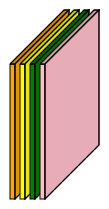
\includegraphics[scale=.5]{conv-feature-maps}}
  \end{figure}
  \begin{description}
  \item[Input] $32 \times 32 \times 3$
  \item[Filtres] $4 \times 6 \times 6 \times 3$
  \item[Output] $27 \times 27 \times 4$
  \end{description}
\end{frame}

\begin{frame}
  \frametitle{Réseau complet typique}
  Entrelacement de couches de convolutions et de non-linéarités:\\
  \begin{figure}
    \raisebox{-0.5\height}{Première couche:}
    \raisebox{-0.5\height}{$\ReLU$}
    \raisebox{-0.5\height}{\Huge(}
    \raisebox{-0.5\height}{
\includegraphics[scale=.2]{conv-filters}}
    \raisebox{-0.5\height}{\huge(}
    \raisebox{-0.5\height}{\includegraphics[scale=.2]{conv-input}}
    \raisebox{-0.5\height}{\huge)}
    \raisebox{-0.5\height}{\Huge)}
    \raisebox{-0.5\height}{=}
    \raisebox{-0.5\height}{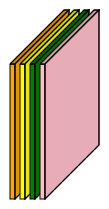
\includegraphics[scale=.2]{conv-feature-maps}}\\
    \raisebox{-0.5\height}{Deuxième couche:}
    \raisebox{-0.5\height}{$\ReLU$}
    \raisebox{-0.5\height}{\Huge(}
    \raisebox{-0.5\height}{
\includegraphics[scale=.2]{conv-filters2}}
    \raisebox{-0.5\height}{\huge(}
    \raisebox{-0.5\height}{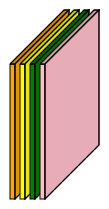
\includegraphics[scale=.2]{conv-feature-maps}}
    \raisebox{-0.5\height}{\huge)}
    \raisebox{-0.5\height}{\Huge)}
    \raisebox{-0.5\height}{=}
    \raisebox{-0.5\height}{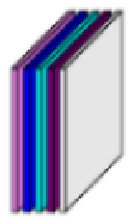
\includegraphics[scale=.2]{conv-feature-maps2}}\\
  \end{figure}
  \begin{table}
    \centering
    \begin{tabular}{lccc}
      \toprule
      Couche & Input &  Filtres & Output \\
      \midrule
      1 & $32 \times 32 \times 3$ & $4 \times 6 \times 6 \times 3$ & $27
                                                                     \times
                                                                     27
                                                                     \times
                                                                     4$
      \\
      2 & $27 \times 27 \times 4$ & $5 \times 4 \times 4 \times 4$ & $24
                                                                     \times
                                                                     24
                                                                     \times
                                                                     5$
      \\
      \bottomrule
      
    \end{tabular}
  \end{table}
  + couches spécifiques à l'output (classification, régression).
\end{frame}

\begin{frame}
  \frametitle{Exercice}
  \begin{description}
  \item[Input] $128 \times 128 \times 3$
  \item[Couche 1] 256 filtres de $5 \times 5 \times ?$
  \item[Couche 2] 512 filtres de $3 \times 3 \times ?$
  \item[Couche 3] 64 filtres de $1 \times 1 \times ?$
  \end{description}
  \begin{enumerate}
  \item Compléter les $?$
  \item Donner la taille de l'output.
  \item Combien de poids contient la dernière couche ?
  \end{enumerate}
\end{frame}

\begin{frame}
  \frametitle{Solution}
  \begin{description}
  \item[Input] $128 \times 128 \times 3$
  \item[Couche 1] 256 filtres de $5 \times 5 \times $\visible<2->{$\red{3}$}
  \item[Couche 2] 512 filtres de $3 \times 3 \times $\visible<3->{$\red{256}$}
  \item[Couche 3] 64 filtres de $1 \times 1 \times $\visible<4->{$\red{512}$}
  \end{description}
  \begin{enumerate}
  \item \visible<1->{Compléter les $?$.}
  \item \visible<5->{Donner la taille de l'output.}\\
    \visible<6->{$128 \times 128 \times 3$}\\
    \visible<7->{→ $124 \times 124 \times 256$}\\
    \visible<8->{→ $122 \times 122 \times 512$}\\
    \visible<9->{→ $122 \times 122 \times 64$}
  \item \visible<10->{Combien de poids contient la dernière couche ?}
    \visible<11->{$1 \times 1 \times 512 \times 64 + 64 = 32832$}
  \end{enumerate}
\end{frame}

\begin{frame}
  \frametitle{Plus de détails sur l'application des filtres}
  Possibilité de modifier l'application des filtres pour construire
  des architectures diverses :
  \begin{itemize}
  \item Stride $n$: Parcourir l'input $n$ par $n$ au lieu de $1$ par
    $1$. Permet de sous-échantillonner.
  \item Padding $n$: Rajouter des $0$ à l'input pour contrôler les
    dimensions de l'output.
  \end{itemize}
  Par exemple, des filtres $5\times5$ avec padding $2$ conservent la taille
  de l'input.
\end{frame}

\begin{frame}
  \frametitle{Exemple de padding}
  Taille $3\times 3$, Stride $1$, padding $1$ sur un input $3 \times
  3$:
  \\[.5cm]
  \begin{tabular}{|c|c|c|c|c|}
    \hline
    \cellcolor{green}0 & \cellcolor{green}0 & \cellcolor{green}0 & 0 & 0 \\
    \hline
    \cellcolor{green}0 & \cellcolor{green}1 & \cellcolor{green}2 & 8 & 0 \\
    \hline
    \cellcolor{green}0 & \cellcolor{green}-7 & \cellcolor{green}-1 & -5 & 0 \\
    \hline
    0 & 3 & 1 & 1 & 0 \\
    \hline
    0 & 0 & 0 & 0 & 0 \\
    \hline
  \end{tabular}
\end{frame}

\begin{frame}
  \frametitle{Exemple de padding}
  Taille $3\times 3$, Stride $1$, padding $1$ sur un input $3 \times
  3$:
  \\[.5cm]
  \begin{tabular}{|c|c|c|c|c|}
    \hline
    0 & \cellcolor{green}0 & \cellcolor{green}0 & \cellcolor{green}0 & 0 \\
    \hline
    0 & \cellcolor{green}1 & \cellcolor{green}2 & \cellcolor{green}8 & 0 \\
    \hline
    0 & \cellcolor{green}-7 & \cellcolor{green}-1 & \cellcolor{green}-5 & 0 \\
    \hline
    0 & 3 & 1 & 1 & 0 \\
    \hline
    0 & 0 & 0 & 0 & 0 \\
    \hline
  \end{tabular}
\end{frame}

\begin{frame}
  \frametitle{Exemple de padding}
  Taille $3\times 3$, Stride $1$, padding $1$ sur un input $3 \times
  3$:
  \\[.5cm]
  \begin{tabular}{|c|c|c|c|c|}
    \hline
    0 & 0 & \cellcolor{green}0 & \cellcolor{green}0 & \cellcolor{green}0 \\
    \hline
    0 & 1 & \cellcolor{green}2 & \cellcolor{green}8 & \cellcolor{green}0 \\
    \hline
    0 & -7 & \cellcolor{green}-1 & \cellcolor{green}-5 & \cellcolor{green}0 \\
    \hline
    0 & 3 & 1 & 1 & 0 \\
    \hline
    0 & 0 & 0 & 0 & 0 \\
    \hline
  \end{tabular}
\end{frame}

\begin{frame}
  \frametitle{Exemple de padding}
  Taille $3\times 3$, Stride $1$, padding $1$ sur un input $3 \times
  3$:
  \\[.5cm]
  \begin{tabular}{|c|c|c|c|c|}
    \hline
    0 & 0 & 0 & 0 & 0 \\
    \hline
    \cellcolor{green}0 & \cellcolor{green}1 & \cellcolor{green}2 & 8 & 0 \\
    \hline
    \cellcolor{green}0 & \cellcolor{green}-7 & \cellcolor{green}-1 & -5 & 0 \\
    \hline
    \cellcolor{green}0 & \cellcolor{green}3 & \cellcolor{green}1 & 1 & 0 \\
    \hline
    0 & 0 & 0 & 0 & 0 \\
    \hline
  \end{tabular}
\end{frame}

\begin{frame}
  \frametitle{Exemple de padding}
  Taille $3\times 3$, Stride $1$, padding $1$ sur un input $3 \times
  3$:
  \\[.5cm]
  \begin{tabular}{|c|c|c|c|c|}
    \hline
    0 & 0 & 0 & 0 & 0 \\
    \hline
    0 & \cellcolor{green}1 & \cellcolor{green}2 & \cellcolor{green}8 & 0 \\
    \hline
    0 & \cellcolor{green}-7 & \cellcolor{green}-1 & \cellcolor{green}-5 & 0 \\
    \hline
    0 & \cellcolor{green}3 & \cellcolor{green}1 & \cellcolor{green}1 & 0 \\
    \hline
    0 & 0 & 0 & 0 & 0 \\
    \hline
  \end{tabular}
\end{frame}

\begin{frame}
  \frametitle{Exemple de padding}
  Taille $3\times 3$, Stride $1$, padding $1$ sur un input $3 \times
  3$:
  \\[.5cm]
  \begin{tabular}{|c|c|c|c|c|}
    \hline
    0 & 0 & 0 & 0 & 0 \\
    \hline
    0 & 1 & \cellcolor{green}2 & \cellcolor{green}8 & \cellcolor{green}0 \\
    \hline
    0 & -7 & \cellcolor{green}-1 & \cellcolor{green}-5 & \cellcolor{green}0 \\
    \hline
    0 & 3 & \cellcolor{green}1 & \cellcolor{green}1 & \cellcolor{green}0 \\
    \hline
    0 & 0 & 0 & 0 & 0 \\
    \hline
  \end{tabular}
\end{frame}

\begin{frame}
  \frametitle{Exemple de padding}
  Taille $3\times 3$, Stride $1$, padding $1$ sur un input $3 \times
  3$:
  \\[.5cm]
  \begin{tabular}{|c|c|c|c|c|}
    \hline
    0 & 0 & 0 & 0 & 0 \\
    \hline
    0 & 1 & 2 & 8 & 0 \\
    \hline
    \cellcolor{green}0 & \cellcolor{green}-7 & \cellcolor{green}-1 & -5 & 0 \\
    \hline
    \cellcolor{green}0 & \cellcolor{green}3 & \cellcolor{green}1 & 1 & 0 \\
    \hline
    \cellcolor{green}0 & \cellcolor{green}0 & \cellcolor{green}0 & 0 & 0 \\
    \hline
  \end{tabular}
\end{frame}

\begin{frame}
  \frametitle{Exemple de padding}
  Taille $3\times 3$, Stride $1$, padding $1$ sur un input $3 \times
  3$:
  \\[.5cm]
  \begin{tabular}{|c|c|c|c|c|}
    \hline
    0 & 0 & 0 & 0 & 0 \\
    \hline
    0 & 1 & 2 & 8 & 0 \\
    \hline
    0 & \cellcolor{green}-7 & \cellcolor{green}-1 & \cellcolor{green}-5 & 0 \\
    \hline
    0 & \cellcolor{green}3 & \cellcolor{green}1 & \cellcolor{green}1 & 0 \\
    \hline
    0 & \cellcolor{green}0 & \cellcolor{green}0 & \cellcolor{green}0 & 0 \\
    \hline
  \end{tabular}
\end{frame}

\begin{frame}
  \frametitle{Exemple de padding}
  Taille $3\times 3$, Stride $1$, padding $1$ sur un input $3 \times
  3$:
  \\[.5cm]
  \begin{tabular}{|c|c|c|c|c|}
    \hline
    0 & 0 & 0 & 0 & 0 \\
    \hline
    0 & 1 & 2 & 8 & 0 \\
    \hline
    0 & -7 & \cellcolor{green}-1 & \cellcolor{green}-5 & \cellcolor{green}0 \\
    \hline
    0 & 3 & \cellcolor{green}1 & \cellcolor{green}1 & \cellcolor{green}0 \\
    \hline
    0 & 0 & \cellcolor{green}0 & \cellcolor{green}0 & \cellcolor{green}0 \\
    \hline
  \end{tabular}
\end{frame}

\begin{frame}
  \frametitle{Exemple de padding}
  Taille $3\times 3$, Stride $1$, padding $1$ sur un input $3 \times
  3$:
  \\[.5cm]
  \begin{tabular}{|c|c|c|c|c|}
    \hline
    0 & 0 & 0 & 0 & 0 \\
    \hline
    0 & 1 & 2 & 8 & 0 \\
    \hline
    0 & -7 & \cellcolor{green}-1 & \cellcolor{green}-5 & \cellcolor{green}0 \\
    \hline
    0 & 3 & \cellcolor{green}1 & \cellcolor{green}1 & \cellcolor{green}0 \\
    \hline
    0 & 0 & \cellcolor{green}0 & \cellcolor{green}0 & \cellcolor{green}0 \\
    \hline
  \end{tabular}

  → L'output conserve la dimension de l'input ($3 \times 3$) malgré la
  taille du filtre > $1$ !
\end{frame}

\begin{frame}
  \frametitle{Exemple de stride}
  Taille $2\times 2$, Stride $2$, padding $0$ sur un input $4 \times
  4$:
  \\[.5cm]
  \begin{tabular}{|c|c|c|c|}
    \hline
    \cellcolor{green}5 & \cellcolor{green}1 & 2 & 8 \\
    \hline
    \cellcolor{green}-1 & \cellcolor{green}-7 & -1 & -5 \\
    \hline
    2 & 3 & 1 & 1 \\
    \hline
    3 & 0 & 1 & 2 \\
    \hline
  \end{tabular}

\end{frame}
\begin{frame}
  \frametitle{Exemple de stride}
  Taille $2\times 2$, Stride $2$, padding $0$ sur un input $4 \times
  4$:
  \\[.5cm]
  \begin{tabular}{|c|c|c|c|}
    \hline
    5 & 1 & \cellcolor{green}2 & \cellcolor{green}8 \\
    \hline
    -1 & -7 & \cellcolor{green}-1 & \cellcolor{green}-5 \\
    \hline
    2 & 3 & 1 & 1 \\
    \hline
    3 & 0 & 1 & 2 \\
    \hline
  \end{tabular}

\end{frame}
\begin{frame}
  \frametitle{Exemple de stride}
  Taille $2\times 2$, Stride $2$, padding $0$ sur un input $4 \times
  4$:
  \\[.5cm]
  \begin{tabular}{|c|c|c|c|}
    \hline
    5 & 1 & 2 & 8 \\
    \hline
    -1 & -7 & -1 & -5 \\
    \hline
    \cellcolor{green}2 & \cellcolor{green}3 & 1 & 1 \\
    \hline
    \cellcolor{green}3 & \cellcolor{green}0 & 1 & 2 \\
    \hline
  \end{tabular}

\end{frame}
\begin{frame}
  \frametitle{Exemple de stride}
  Taille $2\times 2$, Stride $2$, padding $0$ sur un input $4 \times
  4$:
  \\[.5cm]
  \begin{tabular}{|c|c|c|c|}
    \hline
    5 & 1 & 2 & 8 \\
    \hline
    -1 & -7 & -1 & -5 \\
    \hline
    2 & 3 & \cellcolor{green}1 & \cellcolor{green}1 \\
    \hline
    3 & 0 & \cellcolor{green}1 & \cellcolor{green}2 \\
    \hline
  \end{tabular}

\end{frame}

\begin{frame}
  \frametitle{Deux autres blocs utilisés}
  En plus des convolutions et non-linéarités, on utilise:
  \begin{itemize}
  \item Bloc de pooling pour sous-échantillonner
  \item Bloc de normalisation de batch pour améliorer l'apprentissage
  \end{itemize}
\end{frame}

\begin{frame}
  \frametitle{Bloc de pooling}
  \begin{itemize}
  \item Réduit la dimensionnalité du volume en aggrégeant les valeurs
  \item Utilise une moyenne ou un maximum
  \item Pas de paramètres ! Fonction fixe
  \item À contraster avec les convolutions à stride > 1.
  \end{itemize}
\end{frame}

\begin{frame}
  \frametitle{Bloc de pooling}
  Pooling max de taille $2\times 2$, Stride $2$, padding $0$ sur un input $4 \times
  4$:
  \\[.5cm]
  \begin{tabular}{|c|c|c|c|}
    \hline
    \cellcolor{green}5 & \cellcolor{green}1 & 2 & 8 \\
    \hline
    \cellcolor{green}-1 & \cellcolor{green}-7 & -1 & -5 \\
    \hline
    2 & 3 & 1 & 1 \\
    \hline
    3 & 0 & 1 & 2 \\
    \hline
  \end{tabular}

  Résultat:
  \begin{tabular}{|c|c|}
    \hline
    \cellcolor{green}5 & 8 \\
    \hline
    3 & 2 \\
    \hline
  \end{tabular}
\end{frame}
\begin{frame}
  \frametitle{Bloc de pooling}
  Pooling max de taille $2\times 2$, Stride $2$, padding $0$ sur un input $4 \times
  4$:
  \\[.5cm]
  \begin{tabular}{|c|c|c|c|}
    \hline
    5 & 1 & \cellcolor{green}2 & \cellcolor{green}8 \\
    \hline
    -1 & -7 & \cellcolor{green}-1 & \cellcolor{green}-5 \\
    \hline
    2 & 3 & 1 & 1 \\
    \hline
    3 & 0 & 1 & 2 \\
    \hline
  \end{tabular}

  Résultat:
  \begin{tabular}{|c|c|}
    \hline
    5 & \cellcolor{green}8 \\
    \hline
    3 & 2 \\
    \hline
  \end{tabular}
\end{frame}
\begin{frame}
  \frametitle{Bloc de pooling}
  Pooling max de taille $2\times 2$, Stride $2$, padding $0$ sur un input $4 \times
  4$:
  \\[.5cm]
  \begin{tabular}{|c|c|c|c|}
    \hline
    5 & 1 & 2 & 8 \\
    \hline
    -1 & -7 & -1 & -5 \\
    \hline
    \cellcolor{green}2 & \cellcolor{green}3 & 1 & 1 \\
    \hline
    \cellcolor{green}3 & \cellcolor{green}0 & 1 & 2 \\
    \hline
  \end{tabular}

  Résultat:
  \begin{tabular}{|c|c|}
    \hline
    5 & 8 \\
    \hline
    \cellcolor{green}3 & 2 \\
    \hline
  \end{tabular}
\end{frame}
\begin{frame}
  \frametitle{Bloc de pooling}
  Pooling max de taille $2\times 2$, Stride $2$, padding $0$ sur un input $4 \times
  4$:
  \\[.5cm]
  \begin{tabular}{|c|c|c|c|}
    \hline
    5 & 1 & 2 & 8 \\
    \hline
    -1 & -7 & -1 & -5 \\
    \hline
    2 & 3 & \cellcolor{green}1 & \cellcolor{green}1 \\
    \hline
    3 & 0 & \cellcolor{green}1 & \cellcolor{green}2 \\
    \hline
  \end{tabular}

  Résultat:
  \begin{tabular}{|c|c|}
    \hline
    5 & 8 \\
    \hline
    3 & \cellcolor{green}2 \\
    \hline
  \end{tabular}
\end{frame}

\begin{frame}
  \frametitle{Paramètres de pooling}
  \begin{itemize}
  \item $2 \times 2$, stride $2$, padding $0$
  \item $4 \times 4$, stride $2$, padding $1$
  \end{itemize}
\end{frame}

\begin{frame}
  \frametitle{Bloc de normalisation de batch}
  \begin{itemize}
  \item Lutter contre un effet pervers de la rétropropagation des
    gradients~\cite{Ioffe2015}
  \item Facilite grandement l'apprentissage
  \item Utilisé dans tous les modèles récents
  \end{itemize}
\end{frame}

\begin{frame}
  \frametitle{Bloc de normalisation de batch}
  \begin{itemize}
  \item Après un pas de rétropropagation, un layer $n$ change de
    distribution d'output
  \item Le layer $n+1$ a appris sur la distribution d'avant
  \end{itemize}
  → L'entraînement est donc inefficace !
\end{frame}
\begin{frame}
  \frametitle{Bloc de normalisation de batch}
  Solution: normaliser le batch après le layer $n$ pour qu'il soit
  stable pour le layer $n+1$: diviser par sa variance et soustraire sa
  moyenne.
\end{frame}

\begin{frame}
  \frametitle{Conclusion}
  \begin{itemize}
  \item Les convolutions sont des neurones à l'input restreint
  \item Un réseau à convolutions transforme des tenseurs 3d en
    d'autres tenseurs 3d
  \item Le nombre, la taille et l'application des filtres contrôle ces
    transformations
  \item Des non-linéarités, des blocs de poolings et de la
    normalisation par batch sont utilisés en complément des convolutions
  \end{itemize}
\end{frame}

\begin{frame}[allowframebreaks]
  \bibliography{papers}
\end{frame}
\end{document}

%%% Local Variables:
%%% mode: latex
%%% TeX-master: t
%%% End:
